\RequirePackage{shellesc}
\documentclass{scrartcl}
\KOMAoptions
  {
    fontsize=12pt,
    paper=a4,
    pagesize=pdftex,
    DIV=calc,
    headings=standardclasses,
    headings=small,
    twoside=on,
    BCOR=1cm
  }
  
\usepackage{adrianschneider}
\DeclareMathOperator{\sign}{sign}
\DeclareMathOperator{\Langevin}{L}
\newcommand{\He}{H_\text{e}}
\newcommand{\Man}{M_\text{an}}
\newcommand{\Msat}{M_\text{sat}}
\newcommand{\Mirr}{M_\text{irr}}
\newcommand{\Mrev}{M_\text{rev}}
\newcommand{\textref}[1]{\text{(\ref{#1})}}
\newcommand{\eqr}[1]{\underset{\textref{#1}}{=}}
  
\addbibresource{theory.bib}
\begin{document}

\tableofcontents
\newpage
\section{Einleitung}
\subsection{Zielsetzung}
Ziel des Projektes ist es, die Kernverluste in induktiven Bauelementen besser vorhersagen zu können als mit den bisherigen Methoden. Das typische Vorgehen bei der Abschätzung dieser Verluste basiert derzeit meist auf der Steinmetz-Formel bzw. auf ihren Erweiterungen. Diese beschreibt rein phänomenologisch die Verluste abhängig von Flussdichte, Frequenz und Temperatur. Dabei wird jedoch weder die Strom- noch die Kernform einbezogen.\\
\subsection{Hysteresemodelle}
Um hier eine Verbesserung erzielen zu können, ist es notwendig, die Hysterese transient zu beschreiben und mit diesem Modell die Verluste zu berechnen. Die Wissenschaft hat hierfür einige Modelle hervorgebracht:
\begin{labeling}{Krasnosel’skii–Pokrovskii}
	\item[Komplexe Permeabilität]{}
	\item[Jiles-Atherton]{}
	\item[Preisach]{}
	\item[Coleman-Hodgdon]{}
	\item[Krasnosel’skii–Pokrovskii]{}
	\item[Maxwell-Slip]{}
	\item[Bouc–Wen]{}
	\item[Duhem]{}
	\item[VINCH]{}
\end{labeling}
Die verschiednen Modelle unterscheiden sich insbesondere in der Anzahl der Modellparameter. Während das Jiles-Atherton mit fünf Parametern auskommt, können etwa im Preisach- oder VINCH-Modell beliebig viele Parameter eingeführt werden -- dies führt dazu, dass gemessene Hysteresekurven genauer angenähert werden können, jedoch vermutlich die Allgemeingültigkeit ein Stück weit verloren geht.\\
Ein entscheidendes Problem bei fast allen erwähnten Modellen ist die Parameteridentifikation -- die Modellparameter müssen an Messkurven angeglichen werden. Bei dem Modell der komplexen Permeabilität fällt dies noch recht leicht, da hier einer einfachen Leistungsmessung ausreicht (noch dazu ist das Modell linear). Für die anderen Modelle, die alle nichtlinear sind, gestaltet sich dies jedoch deutlich schwieriger.
\subsection{Parameteridentifikation}
Das übliche Vorgehen ist, eine Kostenfunktion aufzustellen, die ihr Minimum dann annimmt, wenn Messdaten und Simulationsdaten am besten übereinstimmen. Diese Kostenfunktion muss anschließend mit einem geeigneten Algorithmus minimiert werden. Für nichtlineare Modelle wie die vorliegenden gestaltet sich dies jedoch oft sehr schwierig -- die meisten Algorithmen benötigen für eine schnelle Konvergenz die Jacobi- oder sogar auch die Hesse-Matrix der zu minimierenden Kostenfunktion. Diese sind analytisch jedoch nicht zugänglich. Ein alternativer Ansatz ist, gradientenfreie Algorithmen zu verwenden (genetische Algorithmen, linear Programming etc.). Dies wurde in der Literatur auch wiederholt vorgenommen -- die Konvergenz kann hierbei jedoch nicht garantiert werden, noch dazu sind diese Algorithmen recht langsam.
\subsection{Automatisches Differenzieren}
Ein Ausweg aus diesen Problemen versprechen die neuen Möglichkeiten aus dem Gebiet des automatischen Differenzierens. Durch die stetige Erhöhung der Rechenleistung von Computern und die neuen Anwendungsmöglichkeiten im Bereich der künstlichen Intelligenz konnten hier in den letzten Jahren viele Verbesserungen erreicht werden.\\
Mit dem automatischen Differenzieren ist es möglich, Computerprogramme abzuleiten, also Jacobi-, Hessematrix etc. für Programmme zu bestimmen. Die Idee hinter diesem Projekt ist es nun, die Fortschritte in diesem Bereich zu nutzen und auf das dargestellte Problem der Parameteridentifikation von Hysteresemodellen anzuwenden.
\subsection{Vorgehen}
\begin{figure}
\caption{Vorgehen zur Parameteridentifikation iim Fall ohne Ortsauflösung.\\Ausgangspunkt sind die konstituierenden Gleichungen des Jiles-Atherton-Modells, aus denen man die Differentialquotienten gewinnen kann, die man für die numerische Integration benötigt.\\
Mit dieser können Hysteresekurven zu gegebenen Parametern erzeugt werden. Die Differenz von erzeugten Hysteresekurven und den Messdaten führen zur Kostenfunktion, die mit der Methode des automatischen Differenzierens nach den Parametern abgeleitet werden kann.\\
Mit einem Minimierungsalgorithmus kann man das Optimierungsproblem lösen und so die Parameter identifizieren.}
\label{fig:vorgehen_skalar}

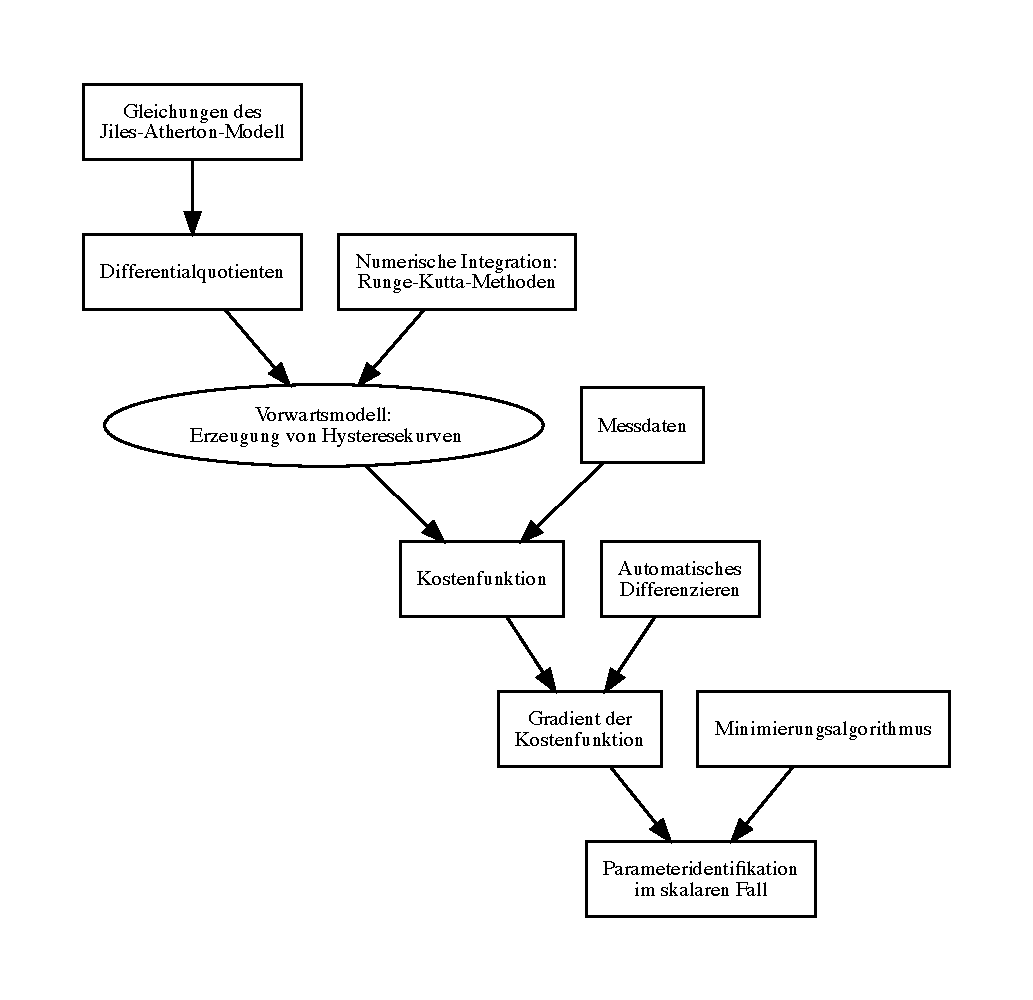
\includegraphics[width=\textwidth]{vorgehen.pdf}

\end{figure}
In Abbildung \ref{fig:vorgehen_skalar} wird das Vorgehen schematisch dargestellt, zumindest der erste Teil es Projektes, die Lösung der Aufgabe im nicht-ortsaufgelösten Fall. Der Projektplan für den zweiten Teil ist im Anhang, Abbildung \ref{fig:vorgehen_ort} bildlich dargestellt.\\
Als Beispielmodell wird das Jiles-Atherton-Modell verwendet, da es relativ populär ist und somit viele Erfahrungswerte in der wissenschaftlichen Literatur vorhanden sind. Außerdem hat es eine recht kleine Parameteranzahl, was einige Vereinfachungen mit sich bringt. Dieses Modell wird in Abschnitt \ref{sec:jiles-atherton} genauer dargestellt.\\
\paragraph{Skalares Vorwärtsmodell} Der nächste Schritt ist, das Vorwärtsmodell für den skalaren Fall (keine Ortsauflösung von Feld und Hysterese) zu entwerfen. Dieses Vorwärtsmodell ist effektiv eine Abbildung vom Parameterraum in die Menge der Hysteresekurven -- für jede Parameterkombination erhält man eine (zeitlich diskretisierte) B-H-Kurve.
\paragraph{Integration} Dies wird durch die Integration der differentiellen Magnetisierung, die das Jiles-Atherton-Modell beschreibt, erreicht. Da die verfügbaren AD-Tools nicht mit den  integrierten Algorithmen der üblichen Mathematik-Pakete umgehen können, muss diese Integration manuell implementiert werden. Als Algorithmus wird ein Runge-Kutta-Verfahren gewählt, welches in einem Fachartikel als geeignet für das Jiles-Atherton-Modell beschrieben wurde. Eine kurze Übersicht zum Thema der numerischen Integration und den Runge-Kutta-Verfahren ist in Abschnitt \ref{sec:numeric-integration} gegeben.
\paragraph{Inverses Problem} Der nächste Schritt ist der Entwurf des inversen Problems: Gesucht ist nun das Urbild einer Hysteresekurve (Messung) im Parameterraum. Dazu wird zuerst eine Kostenfunktion aufgestellt, von der anschließend mit den Methoden des automatischen Differenzierens Jacobi- und Hessematrix ermittelt werden. Daraufhin wird die Kostenfunktion mit einem geeigneten Algorithmus minimiert. Dadurch erhält man die optimierten Parameter zur gegebenen Messkurve.\\
\paragraph{Ortsaufgelöstes Vorwärtsmodell}
Die bisherigen Berechnungen galten stets für ein skalares Modell, der Kern wurde also betrachtet als würde in jedem Punkt das gleiche Feld herrschen. Dies ist jedoch natürlich nur eine Näherung. Daher soll im nächsten Schritt das Jiles-Atherton-Modell auf einen ausgedehnten Kern übertragen werden. Die Zeitdiskretisierung wird genauso wie vorher mit finiten Differenzen (Runge-Kutta-Methode) vorgenommen, die Ortsdiskretisierung basiert auf der Finite-Elemente-Methode. Mit dem ortsaufgelösten Vorwärtsmodell kann nun die Hysterese im gesamten Kern ortsaufgelöst und unter Berücksichtigung der Maxwell-Gleichungen modelliert werden.
\paragraph{Inverses ortsaufgelöstes Problem}
Wie beim skalaren Modell gilt es nun, das inverse Problem zu implementieren. Hierfür wird abermals auf das Automatische Differenzieren zurückgegriffen -- in diesem Fall ist bei einem einzelnen Zeitschritt jedoch nicht eine einzelne Gleichung zu lösen, sondern ein ganzes FEM-Problem. Mit der Software \emph{dolfin-adjoint} kann jedoch die Differenziation von FEM-Modellen abstrahiert und so stark vereinfach werden. Die Kostenfunktion wird nun zu einem Kostenfunktional, also einer Funktion der Lösung der einzelnen FEM-Probleme aus den einzelnen Zeitschritten. Mit einem geeigneten Optimierungssalgorithmus kann nun abermals aus Messwerten auf die Parameter geschlossen werden.
\section{Jiles-Atherton-Modell}
\label{sec:jiles-atherton}
Das Jiles-Atherton-Modell ist ein physikalisch motiviertes Modell zur Beschreibung der Hysterese von magnetischen Materialien.
\subsection{Konstituierende Gleichungen}
\begin{align}
	\He &= H + \alpha M \quad &&\text{Effektives Feld} \label{eq:h_eff}\\
	\Man &= \Msat \Langevin\left(\frac{\He}{a}\right) \quad &&\text{Anhysterische Magnetisierung}  \label{eq:m_an}\\
	\frac{\dif\Mirr}{\dif \He} &= \frac{\Man - \Mirr}{k \sign\left(\frac{\dif H}{\dif t}\right)} \quad &&\text{Pinning} \label{eq:pinning}\\
	M &= \Mrev + \Mirr \quad &&\text{Gesamte Magnetisierung} \label{eq:m_gesamt}\\
	\Mrev &= c(\Man - \Mirr) \quad &&\text{Irreversible Magnetisierung} \label{eq:m_rev}
\end{align}
In diesen fünf Modellgleichungen kommen fünf Modellparameter vor:
\begin{labeling}{$\Msat$}
	\item[$\alpha$]{Interdomänenkopplung}
	\item[$a$]{Domänenwanddichte}
	\item[$\Msat$]{Sättigungsmagnetisierung}
	\item[$k$]{Pinning-Energie}
	\item[$c$]{Magnetisierungsreversibilität}
\end{labeling}
Die Funktion $\Langevin(x)$ ist die sogenannte Langevin-Funktion, die die anhysterische Magnetisierungskurve beschreibt. Sie ist definiert durch
\begin{equation}
	\Langevin(x) = \coth(x) - \frac{1}{x}
\end{equation}
\subsection{Herleitung der Differentiale}
Ziel ist es nun, einen differentiellen Zusammenhang zwischen $B$ und $H$ zu finden. Dazu:
\begin{equation}
	M \underset{\textref{eq:m_gesamt}}{=} \Mrev + \Mirr \underset{\textref{eq:m_rev}}{=} c (\Man - \Mirr) + \Mirr = c\Man + (1-c)\Mirr.
\end{equation}
Es gilt also
\begin{equation}
	\dif M = (1-c) \dif\Mirr + c\dif \Man \label{eq:dm}
\end{equation}
und 
\begin{equation}
	\Mirr = \frac{M - c\Man}{1 - c}.
\end{equation}
Weiterhin stimmt jeweils
\begin{align}
	\dif \Mirr &= \frac{\dif \Mirr}{\dif \He}\dif \He \\
	\dif \Man &= \frac{\dif \Man}{\dif \He}\dif \He\\
	\dif \He & \underset{\textref{eq:h_eff}}{=} \dif H + \alpha \dif M. \label{eq:dHe}
\end{align}
Man erhält nun für $\dif M$ zusammengefasst:
\begin{align}
	\begin{split}
		\dif M &\eqr{eq:dm} (1-c) \dif\Mirr + c\dif \Man \\
				&= (1-c) \frac{\dif \Mirr}{\dif \He}\dif \He + c \frac{\dif \Man}{\dif \He}\dif \He,
	\end{split}
\end{align}
in dieser Darstellung sind nun die aus den konstituierenden Gleichungen \ref{eq:m_an} und \ref{eq:pinning} leicht zugänglichen Größen $\dif \Mirr/\dif \He$ und $\dif \Man/\dif \He$ enthalten.
\begin{align}
	\Rightarrow \frac{\dif M}{\dif \He} &= (1-c) \frac{\dif \Mirr}{\dif \He} + c \frac{\dif \Man}{\dif \He} \label{eq:dm_dhe}
\end{align}
Dabei gilt mit Gleichung \ref{eq:m_an}:
\begin{equation}
	\frac{\dif \Man}{\dif \He} = \frac{\Msat}{a} \frac{\dif \Langevin(\He/a)}{\dif(\He/a)}
\end{equation}
Mit Gleichung \ref{eq:dHe} erhält man:
\begin{equation}
	\begin{aligned}
		\dif M &= \frac{\dif M}{\dif \He}\dif \He \\
		&= \frac{\dif M}{\dif \He}\left(\dif H + \alpha \dif M\right) \\[0.3cm]
		\Rightarrow  \frac{\dif M}{\dif H} &= \frac{\dif M/\dif \He}{1 - \alpha \dif M/\dif \He}
	\end{aligned}
\end{equation}
Aus $B = \mu_0(H + M)$ folgt nun
\begin{equation}
	\dif B = \mu_0 (\dif H + \dif M)
\end{equation}
und somit
\begin{equation}
\begin{aligned}
	\frac{\dif B}{\dif H} &= \mu_0 \left(1 + \frac{\dif M}{\dif H}\right)\\[0.3cm]
	&= \mu_0 \frac{1 + (1-\alpha)\dif M/\dif \He}{1 - \alpha \dif M/\dif \He}. \label{eq:dB_dH}
\end{aligned}
\end{equation}\vspace{0.3cm}
Entsprechend gilt für die vom $B$-Feld abhängige Formulierung
\begin{equation}
	\frac{\dif H}{\dif B} = \frac{1}{\mu_0} \frac{1 - \alpha \dif M/\dif \He}{1 + (1-\alpha)\dif M/\dif \He}
\end{equation}
\paragraph{Abhängigkeiten}
Die Differentiale sind, wenn man alle Terme ausschreibt, abhängig von $B$, $H$, $\dif H/\dif t$ und dem Parametervektor $\vec{p} = (\alpha, a, \Msat, k, c)^T$:
\begin{equation}
	\frac{\dif B}{\dif H} = f\left(B, H, \frac{\dif H}{\dif t}, \vec p \right)
\end{equation}
\section{Numerische Integration}
\label{sec:numeric-integration}
Das Jiles-Atherton-Modell beschreibt -- wie oben gezeigt -- nur einen differentiellen Zusammenhang. Um Aussagen über den zeitlichen Verlauf der Magnetisierung und somit über die Kernverluste zu gewinnen, muss die jeweilige gewöhnliche Differentialgleichung integriert werden, zum Beispiel
\begin{equation}
B(H) = \int \frac{\dif B}{\dif H}\dif H + \text{const.}
\end{equation}
Diese Integration ist analytisch nicht zugänglich und muss numerisch ausgeführt werden. Man verwendet hierfür typischerweise integrierte Lösungen wie den Solver \emph{ode45} in Matlab oder das Python-Äquivalent \emph{scipy.integrate.ode}. Diese Methoden implementieren die üblichen Verfahren, explizit das Runge-Kutta-Fehlberg-Verfahren. Dieses ist eine Variante des klassischen Runge-Kutta-Verfahrens mit adaptiver Schrittweite.\\
Da im Nachfolgenden jedoch das Ergebnis einer solchen Integration nach dem Parametervektor $\vec p$ differenziert werden soll, benötigt man einen Integrationsalgorithmus, der den Werkzeugen der Automatischen Differenziation zugänglich ist. Aus diesem Grund muss die Integration manuell implementiert werden.
\subsection{Explizites Euler-Verfahren}
Das einfachste Integrationsverfahren ist das explizite Euler-Verfahren (Forward-Euler, Polygonzugverfahren), es entspricht dem einfachsten expliziten Finite-Differenzen-Ansatz:
\begin{equation}
\begin{aligned}
	\frac{\dif y}{\dif t} &= f(y, t)\\[0.5cm]
	\Rightarrow	\quad \frac{y_{n} - y_{n-1}}{t_{n} - t_{n-1}} &\approx f(y_{n-1}, t_{n-1})
\end{aligned}
\end{equation}
So erhält man für den jeweils nächsten Zeitschritt
\begin{equation}
	y_n \approx y_{n-1} + f(y_{n-1}, t_{n-1})(t_n - t_{n-1})
\end{equation}
\subsection{Implizites Euler-Verfahren}
Im vorherigen Abschnitt wurde ein explizites Verfahren gewählt, d.h. die Funktion $f(y,t)$ wurde durch bereit bekannte Werte von $y$ und $t$ angenähert, $f(y, t) \approx f(y_{n-1}, t_{n-1})$. Alternativ kann man auch einen impliziten Ansatz wählen, $f(y, t) \approx f(y_n, t_n)$, dann erhält man eine implizite Gleichung für den nächsten Zeitschritt
\begin{equation}
	y_n = y_{n-1} + f(y_n, t_n)(t_n - t_{n-1}).
\end{equation}
Diese Gleichung ist jedoch -- da sie implizit und im Allgemeinen nichtlinear ist -- ungleich schwerer zu lösen als die explizite, man benötigt hier üblicherweise numerische Methoden wie die Fixpunktiteration oder etwa, falls der Gradient vorhanden ist, das Newton-Verfahren.\\
Der erhöhte Rechenaufwand der impliziten Verfahren wird durch eine erhöhte Stabilität ausgeglichen, insbesondere bei der Problemklasse der steifen Probleme.\\
Die Integration des Jiles-Atherton-Modells stellt jedoch keine hohen Anforderungen an die Stabilität, wodurch explizite Verfahren verwendet werden können.
\subsection{Kurzer Vergleich}
Der Nachteil von diesen einfachen Verfahren ist ihre geringe Genauigkeit, bzw. die sehr kleine Schrittweite und somit der erhöhte Rechenaufwand, welche man wählen muss, um eine ausreichende Genauigkeit zu erhalten. Als Beispiel soll nun die wohl einfachste Differentialgleichung
\begin{equation}
	\frac{\dif y}{\dif t} = y(t), \quad y(0) = 1 \label{eq:ode}
\end{equation}
mit der Lösung $y(t) = \E^t$ betrachtet werden.\\
\begin{figure}
\fcapside[\FBwidth]{
\caption{Vergleich von einfachen numerischen Integrationsverfahren (vgl. ODE \ref{eq:ode}). Die durchgezogene Linie ist die exakte Lösung, gepunktet sieht man das Resultat des expliziten Euler-Verfahrens, das implizite Verfahren ist gestrichelt dargestellt. Die vertikalen Gitterlinien beschreiben die diskretisierten Zeiten.}
\label{fig:euler}
}{
	\begin{mplibcode}
input graph;
beginfig(1);
	lx := 0.5*\mpdim{\textwidth};
	ly := 0.5*lx;
	sp := 0.5mm;
	draw begingraph(lx,ly);
	setcoords(linear, linear);
	setrange((0.0, 0.0), 1.1, 3.9);
	
	for y=1 step 1 until 3.5:
   	grid.lft(textext("\footnotesize\num[round-mode = places, round-precision=1]{" & decimal y & "}"), y) withcolor .7white;
	endfor;
	
	for y=0 step 0.2 until 1:
   	grid.bot(textext("\footnotesize\num[round-mode = places, round-precision=1]{" & decimal y & "}"), y) withcolor .7white;
	endfor;
	
	pickup pencircle scaled 0.5bp;
    gdraw "../scripts/data/euler_analytic.txt";
    gdraw "../scripts/data/euler_explicit.txt" dashed dashpattern(on 0.1bp off 2bp);
    gdraw "../scripts/data/euler_implicit.txt" dashed evenly;
	
	pickup pencircle scaled 0.5bp; 
	frame.llft;
    endgraph;
	drawarrow (-sp,0) -- (lx, 0);
	drawarrow (0,-sp) -- (0, ly);
	path bounds;
	bounds := (0, 0) -- (xpart lrcorner currentpicture, 0) -- urcorner currentpicture --(0, ypart ulcorner currentpicture) -- cycle;
	setbounds currentpicture to bounds;
	endfig; 
\end{mplibcode}}
\vspace{0.5cm} 
\end{figure}%
Wie man in Abbildung \ref{fig:euler} erkennt, akkumulieren sich in beiden Verfahren (bei großer Schrittweite) schnell große Fehler. Das explizite Verfahren nutzt die Steigung im aktuellen Punkt für den nächsten Schritt, unterschätzt bei der $\E$-Funktion also stets die Steigung, während das implizite Verfahren jeweils die Steigung im nächsten Punkt als Näherung verwendet. Die führt in diesem Fall jeweils zu einer Überschätzung der Steigung.\par
Um die Schrittweise nicht zu klein wählen zu müssen und somit den Rechenaufwand zu reduzieren, wurden viele verschiedene Integrationsverfahren entworfen. Die meisten sind Einschritt-Verfahren, wie etwa die Runge-Kutta-Methoden -- für den nächsten Zeitschritt werden dabei jedoch Zwischenschritte berechnet, die die Näherung verbessern. Man erhöht so zwar den Aufwand für einen einzelnen Schritt, kann aber dafür die Schrittweite deutlich größer wählen.\\
Eine weitere Möglichkeit, den Rechenaufwand zu reduzieren ist eine adaptive Schrittweitensteuerung: Man schätzt mit einem weiteren Zwischenschritt den Fehler und kann so die Schrittweite jeweils so groß wie möglich wählen (vgl. Runge-Kutta-Fehlberg-Methode).\\
Die Wahl des richtigen Algorithmus ist stets vom genauen Problem abhängig, für die vorliegende Integration des Jiles-Atherton-Modells eignet sich laut \cite{ja-rk} jedoch der viel verwendete RK4-Algorithmus mit fester Schrittweite.
\subsection{Runge-Kutta-Methoden}
Die Euler-Verfahren sind Sonderfälle der Runge-Kutta-Methoden, welche eine wichtige Klasse von Einschrittverfahren darstellen. Der m-stufige Algorithmus benötigt Gewichte $\alpha_i, \gamma_i, 1 \le i \le m$ und $\beta_{i,l}, 1\le i, l\le m$. Weiterhin müssen die Schrittweiten  $h_i$ vorgegeben werden, zur Vereinfachung soll jedoch eine feste Schrittweite $h$ angenommen werden.\\
Für den nächsten Datenpunkt berechnet man:
\begin{equation}
\begin{aligned}
	\text{Nächster Zeitpunkt} && t_n &= t_{n-1} + h \\
	\text{i-ter Hilfswert} && k_i &= f\left(y_{n-1} + h \sum_{l=1}^m \beta_{i,l}k_l, t_{n-1} + \alpha_i h\right) \\
	\text{Nächster Wert} && y_n &= y_{n-1} + h\sum_{l=1}^m y_l k_l
\end{aligned}
\end{equation}
Die Gewichte werden meist in einem sogenannten Butcher-Tableau dargestellt
\begin{equation*}
	\begin{array}{c|ccc}
	\alpha_1 	& \beta_{1,1}   & \cdots & \beta_{1,m} \\
	\alpha_2 	& \beta_{2,1}   & \cdots & \beta_{2,m} \\
	\vdots      & \vdots        & \ddots & \vdots        \\
	\alpha_m    & \beta_{m,1}   & \cdots & \beta_{m,m} \\
	\hline
	            & \gamma_1      & \cdots & \gamma_m
\end{array}.
\end{equation*}
Die entstehenden Gleichungen für die Hilfswerte $k_i$ sind im Allgemeinen implizit, sie müssten also iterativ gelöst werden. Sind jedoch die Werte $k_i$ nur von schon vorher berechneten Werten $k_j, j < i$ abhängig, entsteht ein explizites Verfahren. Die Koeffizienten $\beta_{i,l}$ lassen sich im Butcher-Tableau nun als untere Dreiecksmatrix anordnen -- das klassische Runge-Kutta-Verfahren (RK4) hat beispielsweise das Tableau
\begin{equation}
\renewcommand\arraystretch{1.2}
\begin{array}{c|cccc}
	0 &&&& \\
	\tfrac{1}{2} & \tfrac{1}{2} &&& \\
	\tfrac{1}{2} & 0 & \tfrac{1}{2} && \\
	1 & 0 & 0 & 1 &\\
	\hline
	& \tfrac{1}{6} & \tfrac{1}{3} & \tfrac{1}{3} & \tfrac{1}{6}
\end{array}
\end{equation}
Schreibt man für dieses die einzelnen Schritte aus, so ist die Berechnung des nächsten Wertes im RK4-Verfahren:
\begin{equation}
\label{eq:RK4}
	\begin{aligned}
		t_n &= t_{n-1} + h \\[0.3cm]
		k_1 &= f\left(y_{n-1},{} t_{n-1}\right) \\
		k_2 &= f\left(y_{n-1} + hk_1/2,{} t_{n-1} + h/2\right) \\
		k_3 &= f\left(y_{n-1} + hk_2/2,{} t_{n-1} + h/2\right) \\
		k_4 &= f\left(y_{n-1} + hk_3,{} t_{n-1} + h\right) \\[0.3cm]
		y_n &= y_{n-1} + \tfrac{h}{6}\left(k_1 + 2k_2 + 2k_3 + k_4 \right)
	\end{aligned}
\end{equation}
\subsection{Integration des Jiles-Atherton-Modells}
Genau dieses klassische Runge-Kutta-Verfahren soll nun auf das Jiles-Atherton-Modell angewendet werden. Das Differential $dB/dH$ aus Gleichung \ref{eq:dB_dH} wird nun als die zu integrierende Funktion $f$ betrachtet. Es gilt also
\begin{equation}
	\dif B = f\left(B, H, \tfrac{dH}{dt}, \vec{p}\right)\dif H.
\end{equation}
Als Eigabe benötigt der Algorithmus je ein Array für das magnetische Feld $H$ und für die Zeitpunkte $t$, weiterhin eines für die Parameter. Da das RK4-Verfahren für jeden Schritt auch Funktionsauswertungen bei $t_n + h/2$ benötigt, müssen auch für $H$ Werte bei $t_n + h/2$ vorliegen. Dies wird erreicht, indem die Schritte der Integration jeweils zwei Zeitschritte der Eingabedaten umfassen:
\begin{quote}
	$H_{2n}$ und $B_n$ beschreiben stets den gleichen Zeitpunkt $t_{2n}$. Für $B$ existieren somit nur zu jedem zweiten Zeitpunkt Werte. Das Ergebnis $B$ hat entsprechend nur die halbe Samplingrate der Eingangsdaten.
\end{quote}
Dabei ist wichtig, dass der Zeitpunkt $t_{2n+1}$ stets genau in der Mitte zwischen $t_{2n}$ und $t_{2n+2}$ für alle $n \in \mathbb{N}$ liegt. Da Messdaten typischerweise ohnehin äquidistant vorliegen ist das keine starke Einschränkung.\\
Entsprechend der Definition in \ref{eq:RK4} gilt nun
\begin{equation}
\begin{aligned}
	h &= H_{2n} - H_{2n - 2} \span\span\span\span\span\\[0.5cm]
	k_1 &= f\Big(B_{n-1}, &{} H_{2n-2}, &&{} (\tfrac{dH}{dt})_{2n-2},&&{}\vec{p}\Big)\\[0.2cm]
	k_2 &= f\Big(B_{n-1} + h\tfrac{k_1}{2},&{} H_{2n-1},&&{} (\tfrac{dH}{dt})_{2n-1},&&{}\vec{p}\Big)\\[0.2cm]
	k_3 &= f\Big(B_{n-1} + h\tfrac{k_2}{2},&{} H_{2n-1},&&{} (\tfrac{dH}{dt})_{2n-1},&&{} \vec{p}\Big)\\[0.2cm]
	k_4 &= f\Big(B_{n-1} + h k_3, &{} H_{2n}, &&{} (\tfrac{dH}{dt})_{2n},&&{}\vec{p}\Big)\\[0.5cm]
	B_n &= B_{n-1} + \tfrac{h}{6}(k_1 + 2k_2 + 2k_3 + k_4)  \span\span\span\span\span
\end{aligned}
\end{equation}
Dies beschreibt jeweils einen Schritt des Integrationsverfahrens. Führt man diesen für alle Zeitpunkte durch, erhält man die Magnetisierung $M$ für die gewählte Feldvorgabe $H$ und die Modellparameter $\vec{p}$.\\
Der beschriebene Algorithmus wurde, um eine hohe numerische Effizienz zu erzielen, in der Programmiersprache \emph{C++} implementiert. Dabei wurde jedoch nur die Variante mit dem H-Feld verwendet, da die andere numerisch sehr instabil erschien. Um diese funktionsfähig zu machen muss vermutlich auf implizite Verfahren zurückgegriffen werden. Eine genauere Untersuchung dieses Problems steht jedoch aus.
\subsection{Numerische Details}
Um die Stabilität des Algorithmus zu optimieren, gibt es einige Details, die beachtet werden müssen.
\paragraph{Die Langevin-Funktion}
Die Definition der Langevin-Funktion lautet
\begin{equation}
	\Langevin(x) = \coth(x) - \frac{1}{x},
\end{equation}
die beiden Terme haben jeweils in der Umgebung der $0$ eine Polstelle, sind dabei jedoch etwa gleich groß. Durch die sehr großen Werte, die sich jedoch fast vollständig kompensieren tritt bei numerischen Berechnungen unweigerlich ein Signifikanzverlust auf. Entgegenwirken kann man diesem durch eine Approximation in der Nähe der $0$. Es gilt laut \cite{abramowitz}
\begin{equation}
	\coth(x) \approx \frac{1}{x} + \frac{x}{3} - \frac{x^3}{45} + \cdots,
\end{equation}
für die Langevinfunktion folgt also in der Nähe der $0$
\begin{equation}
	\Langevin(x) \approx \frac{x}{3}.
\end{equation}
Entsprechend folgt für die Ableitung:
\begin{equation}
	\frac{\dif \Langevin(x)}{\dif x} = \frac{1}{x^2} - \frac{1}{\sinh(x)^2} \approx \frac{1}{3} - \frac{1}{15}x^2 + \cdots
\end{equation}
\section{Anwendung des Jiles-Atherton-Modells}
Im folgenden Abschnitt sollen nun einige simulierte Kurven präsentiert und anhand dieser die Eigenschaften des Modells erläutert werden.
\begin{figure}[h]
\fcapside[\FBwidth]{\caption[Hystereseschar]{Schar von Hysteresekurven für verschiedene Aussteuerungen. Der nicht-hysterische Teil wird von der Langevinfunktion festgelegt.}\label{fig:hysterseschar}}{
	
\begin{mplibcode}
input graph;
beginfig(1);
	lx := \mpdim{\textwidth}/2.2;
	ly := 3cm;
	pickup pencircle scaled 0.3bp;
	ahlength := 1mm;
	drawarrow (0,ly/2) -- (lx, ly/2);
	drawarrow (lx/2,0) -- (lx/2, ly);
	label.urt(textext("\footnotesize $B$"), (lx/2, ly));
	label.lrt(textext("\footnotesize $H$"), (lx, ly/2));
	draw begingraph(lx,ly);
    gdraw "data/hysteresis1.txt";
    gdraw "data/hysteresis2.txt";
    gdraw "data/hysteresis3.txt";
    gdraw "data/hysteresis4.txt";
    gdraw "data/hysteresis5.txt";
    gdraw "data/hysteresis6.txt";
    gdraw "data/hysteresis7.txt";
	itick.lft(textext(""),0) withcolor white;
	frame.lft withcolor white;
	endgraph;
	path bounds;
	bounds := (0, ypart llcorner currentpicture) -- lrcorner currentpicture -- urcorner currentpicture --(0, ypart ulcorner currentpicture) -- cycle;
	setbounds currentpicture to bounds;
endfig;
\end{mplibcode}
}
\end{figure}
\paragraph{Hysteresekurven} Als erstes Beispiel dient eine Kurvenschar, die Hysteresekurven für verschiedene Aussteuerungen zeigt (Abbildung \ref{fig:hysterseschar}). Man erkennt, dass das Modell die Charakteristik typischer ferromagnetischer Hysteresekurven nachbildet:\\
Bei hohen Feldstärken wächst die Induktion stark an, dies ist die typische Sättigungserscheinung bei Kernmaterialien. Nachdem der Umkehrpunkt erreicht wurde, läuft die Kurve auf einem anderen Weg zurück (Hyterese), sodass die Flussdichte bei verschwindender Feldstärke nicht mehr den Wert $0$ annimmt, sondern eine Restmagnetisierung (Remanenz) übrig bleibt. Im weiteren Verlauf kreuzt die Flussdichte nun die $H$-Achse, den entsprechenden Achsenabschnitt nennt man Koerzitivfeldstärke.
\begin{figure}[h]
\fcapside[\FBwidth]{\caption[Hystereseschar]{Einzelne Hysteresekurve mit Neukurve. }\label{fig:single_curve}}{
	
\begin{mplibcode}
input graph;
beginfig(1);
	lx := \mpdim{\textwidth}/2.2;
	ly := 3cm;
	pickup pencircle scaled 0.3bp;
	ahlength := 1mm;
	drawarrow (0,ly/2) -- (lx, ly/2);
	drawarrow (lx/2,0) -- (lx/2, ly);
	pickup pencircle scaled 0.5bp;
	label.urt(textext("\footnotesize $B$"), (lx/2, ly));
	label.lrt(textext("\footnotesize $H$"), (lx, ly/2));
	draw begingraph(lx,ly);
    gdraw "data/single_hysteresis.txt";
	itick.lft(textext(""),0) withcolor white;
	frame.llft withcolor white;
	endgraph;
	path bounds;
	bounds := (0, ypart llcorner currentpicture) -- lrcorner currentpicture -- urcorner currentpicture --(0, ypart ulcorner currentpicture) -- cycle;
	setbounds currentpicture to bounds;
endfig;
\end{mplibcode}
}
\end{figure}
\par In Abbildung \ref{fig:single_curve} ist eine einzelne Hysteresekurve gezeigt. In diesem Fall ist auch die Neukurve dargestellt, die vom Modell ebenfalls repliziert wird. Im Gegensatz zu den meisten Messkurven beginnt die Neukurve im Jiles-Atherton-Modell jedoch näherungsweise linear. 
\subsection{Stromanregung}
Wie oben gezeigt, kann man entweder $\dif B/\dif H$ oder $\dif H/\dif B$ integrieren. Gibt man einen Strom vor, so ist $\dif H$ festgelegt, man verwendet also $\dif B/\dif H$. Wird der Kern mit einer Spannung angeregt, nutzt man $\dif H/\dif B$. Im Allgemeinen wird man den Kern ohnehin eingebettet in einem Netzwerk betrachten und auch die Integration entsprechend anpassen.\\
\begin{figure}[h]
\fcapside[\FBwidth]{\caption{Verlauf von $H$- und $B$-Feld bei sinusförmiger Stromanregung. Durch die nichtlinearen Kerneigenschaften wird die Form des Sinus stark verbreitert, entsprechend treten hohe Steigungen bei den Nulldurchgängen der magnetischen Flussdichte auf.}\label{fig:current_hb}}{
	
\begin{mplibcode}
input graph;
beginfig(1);
	lx := \mpdim{\textwidth}/2.2;
	ly := 3cm;
	pickup pencircle scaled 0.3bp;
	ahlength := 1mm;
	drawarrow (0,ly/2) -- (lx, ly/2);
	drawarrow (lx/2,0) -- (lx/2, ly);
	pickup pencircle scaled 0.5bp;
	label.urt(textext("\footnotesize $H_\text{norm}$, $B_\text{norm}$"), (lx/2, ly));
	label.lrt(textext("\footnotesize $t$"), (lx, ly/2));
	draw begingraph(lx,ly);
    gdraw "data/stromanregung/current_b.txt" dashed evenly;
    gdraw "data/stromanregung/current_h.txt";
	itick.lft(textext(""),0) withcolor white;
	frame.llft withcolor white;
	endgraph;
	
	picture legend;
	legend = image(
	label.rt(textext("\footnotesize H-Feld"), (0.7*lx, 0.3*ly));
	label.rt(textext("\footnotesize B-Feld"), (0.7*lx, 0.15*ly));
	draw (0.60*lx, 0.3*ly) -- (0.65*lx, 0.3*ly);
	draw (0.60*lx, 0.15*ly) -- (0.65*lx, 0.15*ly) dashed evenly;
	);
	unfill bbox legend;
	draw bbox legend withpen pencircle scaled 0.1bp;
	draw legend;

	path bounds;
	bounds := (0, ypart llcorner currentpicture) -- lrcorner currentpicture -- urcorner currentpicture --(0, ypart ulcorner currentpicture) -- cycle;
	setbounds currentpicture to bounds;
endfig;
\end{mplibcode}
}
\end{figure}

\begin{figure}[h]
\fcapside[\FBwidth]{\caption{Verlauf von Strom und Spannung bei sinusförmiger Stromanregung. Die steilen Flanken der Hysteresekurve führen zu großen Spannungsspitzen durch $\rot E = - \partial B/\partial t$.}\label{fig:current_ui}}{
	
\begin{mplibcode}
input graph;
beginfig(1);
	lx := \mpdim{\textwidth}/2.2;
	ly := 3cm;
	pickup pencircle scaled 0.3bp;
	ahlength := 1mm;
	drawarrow (0,ly/2) -- (lx, ly/2);
	drawarrow (lx/2,0) -- (lx/2, ly);
	pickup pencircle scaled 0.5bp;
	label.urt(textext("\footnotesize $i_\text{norm}$, $u_\text{norm}$"), (lx/2, ly));
	label.lrt(textext("\footnotesize $t$"), (lx, ly/2));
	draw begingraph(lx,ly);
    gdraw "data/stromanregung/current_u.txt" dashed evenly;
    gdraw "data/stromanregung/current_h.txt";
	itick.lft(textext(""),0) withcolor white;
	frame.llft withcolor white;
	endgraph;
	
	picture legend;
	legend = image(
	label.rt(textext("\footnotesize Strom"), (0.7*lx, 0.3*ly));
	label.rt(textext("\footnotesize Spannung"), (0.7*lx, 0.15*ly));
	draw (0.60*lx, 0.3*ly) -- (0.65*lx, 0.3*ly);
	draw (0.60*lx, 0.15*ly) -- (0.65*lx, 0.15*ly) dashed evenly;
	);
	unfill bbox legend;
	draw bbox legend withpen pencircle scaled 0.1bp;
	draw legend;

	path bounds;
	bounds := (0, ypart llcorner currentpicture) -- lrcorner currentpicture -- urcorner currentpicture --(0, ypart ulcorner currentpicture) -- cycle;
	setbounds currentpicture to bounds;
endfig;
\end{mplibcode}
}
\end{figure}

In Abbildung ist der Verlauf von $B$ und $H$-Feld bei Anregung mit einem sinusförmigen Strom gezeigt -- die Sättigungscharakteristik rundet die Spitzen des Sinus deutlich ab, je mehr die Aussteuerung in die Sättigung geht, desto mehr nähert sich die zeitliche Form des $B$-Feldes einer Rechteckschwingung an.\\
Da das Induktionsgesetz die induzierte Spannung mit der zeitlichen Ableitung der magnetischen Flussdichte verknüpft, wird deutlich, dass hier Probleme mit Überpannungen auftreten können -- die steilen Flanken im Verlauf des $B$-Feldes führen zu Spannungsspitzen, die die Isolation des induktiven Bauelements beschädigen können.\par
Die Anregung mit Strömen tritt in der Praxis nur selten auf, weshalb dieses Problem nur in einigen Spezialfällen Probleme verursachen dürfte, ein Beispiel wären Stromwandler, die sehr große Wechselströme heruntertransformieren, um sie Messgeräten zuzuführen.
\subsection{Spannungsanregung}
Der weitaus üblichere Fall ist, dass der Kern näherungsweise von einer Spannungsquelle angeregt wird. Dies ist etwa der typische Fall in einem Transformator, bei dem der Magnetisierungsstrom in erster Näherung von der Primärspannung abhängt.
\begin{figure}[h]
\fcapside[\FBwidth]{\caption{Verlauf von $H$- und $B$-Feld bei sinusförmiger Spannungsanregung. Der typische Verlauf des Magnetisierungsverlauf wird deutlich -- kommt die Induktion in die Nähe der Sättigung, steigt das $H$-Feld und somit der Strom stark an.}\label{fig:voltage_hb}}{
	
\begin{mplibcode}
input graph;
beginfig(1);
	lx := \mpdim{\textwidth}/2.2;
	ly := 3cm;
	pickup pencircle scaled 0.3bp;
	ahlength := 1mm;
	drawarrow (0,ly/2) -- (lx, ly/2);
	drawarrow (lx/2,0) -- (lx/2, ly);
	pickup pencircle scaled 0.5bp;
	label.urt(textext("\footnotesize $H_\text{norm}$, $B_\text{norm}$"), (lx/2, ly));
	label.lrt(textext("\footnotesize $t$"), (lx, ly/2));
	draw begingraph(lx,ly);
    gdraw "data/spannungsanregung/voltage_b.txt" dashed evenly;
    gdraw "data/spannungsanregung/voltage_h.txt";
	itick.lft(textext(""),0) withcolor white;
	frame.llft withcolor white;
	endgraph;
	
	picture legend;
	legend = image(
	label.rt(textext("\footnotesize H-Feld"), (0.7*lx, 0.3*ly));
	label.rt(textext("\footnotesize B-Feld"), (0.7*lx, 0.15*ly));
	draw (0.60*lx, 0.3*ly) -- (0.65*lx, 0.3*ly);
	draw (0.60*lx, 0.15*ly) -- (0.65*lx, 0.15*ly) dashed evenly;
	);
	unfill bbox legend;
	draw bbox legend withpen pencircle scaled 0.1bp;
	draw legend;

	path bounds;
	bounds := (0, ypart llcorner currentpicture) -- lrcorner currentpicture -- urcorner currentpicture --(0, ypart ulcorner currentpicture) -- cycle;
	setbounds currentpicture to bounds;
endfig;
\end{mplibcode}
}
\end{figure}

\begin{figure}[h]
\fcapside[\FBwidth]{\caption{Verlauf von Strom und Spannung bei sinusförmiger Spannungsanregung.}\label{fig:current_ui}}{
	
\begin{mplibcode}
input graph;
beginfig(1);
	lx := \mpdim{\textwidth}/2.2;
	ly := 3cm;
	pickup pencircle scaled 0.3bp;
	ahlength := 1mm;
	drawarrow (0,ly/2) -- (lx, ly/2);
	drawarrow (lx/2,0) -- (lx/2, ly);
	pickup pencircle scaled 0.5bp;
	label.urt(textext("\footnotesize $i_\text{norm}$, $u_\text{norm}$"), (lx/2, ly));
	label.lrt(textext("\footnotesize $t$"), (lx, ly/2));
	draw begingraph(lx,ly);
    gdraw "data/spannungsanregung/voltage_u.txt" dashed evenly;
    gdraw "data/spannungsanregung/voltage_h.txt";
	itick.lft(textext(""),0) withcolor white;
	frame.llft withcolor white;
	endgraph;
	
	picture legend;
	legend = image(
	label.rt(textext("\footnotesize Strom"), (0.7*lx, 0.3*ly));
	label.rt(textext("\footnotesize Spannung"), (0.7*lx, 0.15*ly));
	draw (0.60*lx, 0.3*ly) -- (0.65*lx, 0.3*ly);
	draw (0.60*lx, 0.15*ly) -- (0.65*lx, 0.15*ly) dashed evenly;
	);
	unfill bbox legend;
	draw bbox legend withpen pencircle scaled 0.1bp;
	draw legend;

	path bounds;
	bounds := (0, ypart llcorner currentpicture) -- lrcorner currentpicture -- urcorner currentpicture --(0, ypart ulcorner currentpicture) -- cycle;
	setbounds currentpicture to bounds;
endfig;
\end{mplibcode}
}
\end{figure}
Wie man in den Abbildungen oder auch den Hysteresekurven sieht, wächst der Strom für hohe Induktionen extrem stark an, die Sättigung tritt ein und verursacht enorm hohe Verluste in den Leitern. Daher muss dieser Zustand bei der Auslegung von induktiven Bauelementen im Allgemeinen unbedingt vermieden werden.
\subsection{Allgemeiner Fall}
Im allgemeinen Fall kann man das induktive Bauelement natürlich nicht isoliert betrachten. Vielmehr muss man das Modell des Kerns in ein allgemeines Schaltungsmodell einbinden und dieses transient lösen. So kann man dann auch diverse Themen wie das Einschaltverhalten, das Schaltungsverhalten an der Grenze zur Sättigung oder die Kernverluste im Betrieb untersuchen.
\section{Parameteridentifikation}
Wie am Anfang beschrieben wurde, ist das Ziel dieses Projektes einerseits, das Jiles-Atherton zu untersuchen, andererseits aber vor allem, eine neue Möglichkeit zu finden, um die Modellparameter aus Messdaten zu extrahieren.\\
Der neue Ansatz ist hierbei, die Methoden des algorithmischen Differenzierens zu nutzen, um Jacobi- und Hesse-Matrix für Optimierungsalgorithmen bereitzustellen.
\subsection{Least-Squares-Methode}
Die Standardmethode um Modelle an Messdaten anzupassen, ist die Methode der kleinsten Fehlerquadrate:\\
Man nimmt an, dass die beste Übereinstimmung von Modell und Messung gegeben ist, wenn die Summe der quadratischen Abweichungen minimal ist. Ist $f(\vec x, \vec p)$ die Modellfunktion, die von Eingangswerten $\vec x$ und Parametern $\vec p$ abhängt, so muss man das Minimum der Kostenfunktion
\begin{equation}
	\text{cost}(\vec p) = \sum_i \left(f(x_i, \vec p)-y_i\right)^2
\end{equation}
finden, um die beste Übereinstimmung des Modells mit den gemessenen Daten $\vec y$ zu erhalten.\\
Die zu lösende mathematische Aufgabe ist also die Minimierung einer im Allgemeinen nichtlinearen und nicht konvexen Funktion. Für die Lösung dieser Problemstellung wurden diverse Algorithmen entworfen, die sich grob in zwei Klassen unterteilen lassen können: Ableitungsfreie Methoden und Methoden, die  Ableitungen -- zumindest die Erste -- der zu minimierenden Funktion benötigen.\\
Im Allgemeinen sind Methoden, die Ableitungen nutzen, erfolgreicher, da sie für den nächsten Optimierungsschritt jeweils über Informationen verfügen, in welcher Richtung der Umgebung des aktuellen Schätzwertes die Kostenfunktion am steilsten abfällt. So kann insbesondere die Zahl der Funktionsauswertungen reduziert werden, was insbesondere dann relevant ist, wenn die Funktion rechnerisch teuer ist. Daher kommen gradientenfreie Verfahren üblicherweise erst dann zum Einsatz, wenn Gradientenverfahren nicht mehr einsetzbar sind -- dies ist dann der Fall, wenn Informationen über die Ableitungen nur schwer zu erhalten sind.
\subsection{Probleme bei der Parameteridentifikation für das Jiles-Atherton-Modell}
In der Literatur zum Jiles-Atherton-Modell finden sich viele Ansätze, um mittels gradientenfreier Verfahren auf die Parameter zu schließen. Bei fast all diesen Ansätzen gibt es jedoch ein entscheidendes Problem: Die Geometrie der Probe wird schlicht vernachlässigt -- während man dies bei toroidförmigen Kernen herausrechnen kann, führt es bei Kernen mit keiner derartig großen Symmetrie zu Fehlern. Dies wirkt sich insbesondere auf die Messung von Schichtblech- und Schnittbandkernen aus, da diese nicht toroidförmig erhältlich sind.\\
Die Hysteresekurve wird in solchen Geometrien an verschiedenen Punkten im Material mit verschiedenen Phasenlagen und Amplituden durchlaufen, die messbaren Größen, Spannung und Strom, lassen somit nur einen Schluss auf die integrale und somit geometrieabhängige Hysteresekurve zu.\par
Ziel dieser Arbeit ist es nun, die Geometrie in die Rechnung einzubeziehen. Dazu muss das Jiles-Atherton-Modell in eine orts- und zeitaufgelöste Simulation integriert werden (vgl. \cite{sadowski}, \cite{Bergqvist}), anschließend müssen Strom und Spannung aus dem Modell gewonnen und mit den Messdaten in die Kostenfunktion überführt werden.\\
Offensichtlich ist nun die ursprünglich numerisch wenig aufwändige Funktionsauswertung des Vorwärtsmodells um Größenordnungen teurer geworden. Ein gradientenfreies Verfahren, welches eine kleinere Konvergenzrate hat, dafür aber keine Gradienten berechnen muss, kommt nun nicht mehr infrage -- die Zahl der Funktionsauswertungen ist um Größenordnungen größer als bei Gradientenverfahren.\par
Um das Ziel der Parameteridentifikation unter Beachtung der Geometrie zu ermöglichen, muss also eine Möglichkeit gefunden werden, die Ableitung(en) der Kostenfunktion zu bestimmen. Dafür gibt es drei Möglichkeiten:
\begin{itemize}
	\item Symbolische Berechnung
	\item Numerische Berechnung (Differenzenquotienten)
	\item Automatisches Differenzieren
\end{itemize}
Um die Ableitungen symbolisch zu bestimmen, müssten die relativ komplizierten Gleichungen einzeln differenziert und die jeweiligen Funktionen ebenfalls in den Programmcode geschrieben werden. Dies stellt gerade bei großer Parameterzahl einen enormen Entwicklungsaufwand dar, ist fehleranfällig und meist relativ ineffizient.\\
Die Effizienz ist bei der Berechnung mittels Differenzenquotienten kein Problem -- sie ist hier besonders hoch. Im Kontrast dazu ist jedoch die Genauigkeit sehr klein: Ist die Schrittweite sehr klein, liegen die zwei Funktionswerte eines Quotienten sehr nah beieinander -- dies kann z.B. dazu führen, dass sich zwei Zahlen, die jeweils \SI{32}{\Bit} breit sind, nur in den letzten 5 Stellen unterscheiden. Ein enormer Genauigkeitsverlust ist die Folge.\par
Einen Mittelweg zwischen Geschwindigkeit und Genauigkeit bietet die dritte Methode, das automatische Differenzieren.
\section{Automatisches Differenzieren}
Die Grundidee des automatischen Differenzierens ist relativ simpel: Die Ableitung einer gegebenen Funktion wird mithilfe der Kettenregel so lange umgeformt, bis nur noch Basisfunktionen vorkommen, für die die Ableitung hinterlegt ist.\\
Man unterscheidet zwischen zwei grundlegenden Vorgehensweisen, \emph{Forward-} und dem \emph{Reverse-Mode}.
Um den Unterschied zwischen diesen zu veranschaulichen betrachten wir die Funktion 
\begin{equation}
f(x_1, x_2) = \frac{\sin(x_1/x_2)}{\exp(x_1/x_2)}. \label{eq:example_func}
\end{equation}
Es ist klar einsehbar, dass man diese Funktion als Graph darstellen kann, der die Abfolge der einzelnen Rechenschritte veranschaulicht: Die Kanten stellen Eingangs- und Zwischenwerte dar, die Knoten die Rechenoperatoren. Der Graph ist in Abbildung \ref{fig:computational_graph} dargestellt. Für die Zwischenwerte gilt:
\begin{equation*}
\begin{aligned}
	v_1 &= \frac{x_1}{x_2} &
	v_2 &= \sin(v_1) \\
	v_3 &= \exp(v_1) &
	f = v_4 &= \frac{v_2}{v_3}
\end{aligned}
\end{equation*}\begin{figure}[t]
\fcapside[\FBwidth]{
	\caption{
	Darstellung der Beispielfunktion aus Gleichung \ref{eq:example_func} als Rechengraph (\emph{computational graph}). Es gilt $v_1 = x_1 / x_2$, $v_2 = \sin(v_1)$, $v_3 = \exp(v_1)$ und $v_4 = v_2/v_3$.
	}
	\label{fig:computational_graph}
}{
\begin{tikzpicture}[line join=bevel,scale=0.5]
%%
\node (div2) at (63.0bp,104.0bp) [draw,ellipse] {div};
  \node (result) at (63.0bp,18.0bp) [draw,rectangle] {result};
  \node (exp) at (99.0bp,190.0bp) [draw,ellipse] {exp};
  \node (x2) at (99.0bp,362.0bp) [draw,rectangle] {$x_2$};
  \node (div) at (63.0bp,276.0bp) [draw,ellipse] {div};
  \node (x1) at (27.0bp,362.0bp) [draw,rectangle] {$x_1$};
  \node (sin) at (27.0bp,190.0bp) [draw,ellipse] {sin};
  \draw [->] (x1) -- (div) node [midway, left] {$x_1$};
  \draw [->] (sin) -- (div2) node [midway, left] {$v_2$};
  \draw [->] (div) -- (sin) node [midway, left] {$v_1$};
  \draw [->] (div) -- (exp) node [midway, right] {$v_1$};
  \draw [->] (x2) -- (div) node [midway, right] {$x_2$};
  \draw [->] (div2) -- (result) node [midway, right] {$v_4$};
  \draw [->] (exp) -- (div2) node [midway, right] {$v_3$};
%
\end{tikzpicture}
}
\end{figure}
Aufgabe ist es nun, aus diesem Graphen die Ableitung der Funktion (also dem Wert $v_4$) nach den Eingangsparametern $x_1$ und $x_2$ zu bestimmen. Für die Anwendung der beiden im Folgenden dargestellten Algorithmen müssen neben der Struktur der Funktion lediglich die Ableitungen der Operatoren (runde Knoten) bekannt sein. Es gilt:
\begin{equation*}
\begin{aligned}
	\tfrac{\partial v_1}{\partial x_1} &= \tfrac{1}{x_2} &
	\tfrac{\partial v_1}{\partial x_2} &= -\tfrac{x_1}{x_2^2} &
	\tfrac{\partial v_2}{\partial v_1} &= \cos(v_1) \\
	\tfrac{\partial v_3}{\partial v_2} &= \exp(v_2) &
	\tfrac{\partial v_4}{\partial v_2} &= \tfrac{1}{v_3} &
	\tfrac{\partial v_4}{\partial v_3} &= -\tfrac{v_2}{v_3^2}.
\end{aligned}
\end{equation*}
Diese Ableitungen müssen hinterlegt werden. Da die Basisfunktionen jedoch in den meisten Fällen aus einer relativ kleinen Gruppe stammen, sind diese in den Paketen für automatische Differentiation meistens schon definiert. Für Funktionen, die darüber hinaus gehen, müssen der Operator und seine Ableitung bzw. Ableitungen registriert werden.
\subsection{Forward Mode}

Im \emph{Forward-Mode} wertet man die Funktion nun genauso aus wie sonst -- bezüglich der Klammern von innen nach außen. Dabei notiert man jedoch auch neben der Funktion stets die Ableitungen der einzelnen Ausdrücke. Soll beispielsweise die Ableitung nach $x_2$ im Punkt $(1,2)$ ermittelt werden:
\begin{equation*}
\begin{aligned}
	x_1 &&= 1\\
	\dot{x}_1 &&= 0\\[0.3cm]
	x_2 &&= 2\\
	\dot{x}_2 &&= 1\\[0.3cm]
	v_1 &= x_1/x_2 &= \num{0,5} \\
	\dot{v}_1 &= \tfrac{\partial v_1}{\partial x_1}\dot{x}_1 + \tfrac{\partial v_1}{\partial x_2}\dot{x}_2 = \tfrac{1}{x_2}\dot{x}_1 - \tfrac{x_1}{x_2^2}\dot{x}_2 = \tfrac{1}{2}0 - \tfrac{1}{2^2}1 &= \num{-0,25}\\[0.3cm]
	v_2 &= \sin(v_1) = \sin(1/2) &= \num{0.479425539}\\
	\dot{v}_2 &= \tfrac{\partial v_2}{\partial v_1}\dot{v}_1 = \cos(v_1)\dot v_1 = \cos(\num{0,5})(-\num{0,25}) &= \num{0.219395640}\\[0.3cm]
	v_3 &= \exp(v_1) &= \num{1.648721271}\\
	\dot v_3 &= \tfrac{\partial v_3}{\partial v_1}\dot v_1 = \exp(v_1)\dot v_1 &= \num{-0.412180317} \\[0.3cm]
	v_4 &= \tfrac{v_2}{v_3} &= \num{0.290786288} \\
	\dot v_4 &= \tfrac{\partial v_4}{\partial v_2} \dot v_2 + \tfrac{\partial v_4}{\partial v_3}\dot v_3 = \tfrac{1}{v_3}\dot v_2 - \tfrac{v_2}{v_3^2}\dot v_3 &= \num{-0.060373610}
\end{aligned}
\end{equation*}
Wie man sieht, tritt durch das Differenzieren kein Signifikanzverlust auf, wie bei der Verwendung von Differenzenquotienten. Weiterhin ist der Algorithmus relativ einfach und somit nicht viel langsamer als die Berechnung der Ableitungen mit Differenzenquotienten. Das algorithmische Differenzieren schafft also den oben genannten Mittelweg zwischen symbolischer Differenziation und numerischer Differenziation, den Mittelweg zwischen Genauigkeit und Geschwindigkeit.\par
Der dargestellte Algorithmus weist jedoch im Fall großer Parameterzahlen einen Nachteil auf: Bei jedem Zwischenschritt muss sowohl die Funktionsauswertung selbst, als auch die Ableitung nach jedem Parameter gespeichert werden. Bei großen Parameterzahlen wird der Algorithmus viel Speicher und Rechenleistung brauchen, die Rechenzeit skaliert mit der Parameterzahl.
\subsection{Reverse Mode}
Einen Ausweg aus diesem Problem bietet der zweite Basisalgorithmus des automatischen Differenzierens, der \emph{Reverse Mode}. Bei diesem steigt der Aufwand für Ableitungen nach zusätzlichen Parametern nicht an, wie das folgende Beispiel deutlich macht. Als Funktion wird wieder die aus Gleichung \ref{eq:example_func} betrachtet. Wie der Name \emph{Reverse Mode} sagt, wird der Informationsfluss für die Gradientenbildung rückwärts durchschritten. Damit dies möglich ist, muss also die Funktion vorher einmal in Vorwärtsrichtung ausgeführt und alle Zwischenwerte aufgenommen worden sein. Es gilt also:
\begin{equation*}
	\begin{aligned}
		x_1 &= 1 \\
		x_2 &= 2 \\
		v_1 &= \num{0,5} \\
		v_2 &= \num{0.479425539} \\
		v_3 &= \num{1.648721271} \\
		f = v_4 &= \num{0.290786288} \\[0.5cm]
		\dif f &= \tfrac{\partial f}{\partial v_2} \dif v_2 +  \tfrac{\partial f}{\partial v_3} \dif v_3 \\
		\dif v_2 &= \tfrac{\partial v_2}{\partial v_1} \dif v_1 = \cos(v_1) \dif v_1 \\
		\dif v_3 &= \tfrac{\partial v_3}{\partial v_1} \dif v_1 = \exp(v_1) \dif v_1 \\
		\dif v_1 &= \tfrac{\partial v_1}{\partial x_1} \dif x_1 + \tfrac{\partial v_1}{\partial x_2} \dif x_2 = \tfrac{1}{x_2} \dif x_1 - \tfrac{x_1}{x_2^2} \dif x_2
	\end{aligned}
\end{equation*}
Zusammengefasst folgt
\begin{equation}
	\dif f = \frac{1}{v_3}\cos(v_1)\left(\frac{1}{x_2} \dif x_1 - \frac{x_1}{x_2^2}\dif x_2\right) - \frac{v_2}{v_3^2}\exp(v_1)\left(\frac{1}{x_2}\dif x_1 - \frac{x_1}{x_2^2}\dif x_2\right).
\end{equation}
Wie man sieht, erhält man sofort die Ableitungen nach den beiden Parametern:
\begin{equation}
	\frac{\dif f}{\dif x_1} = \frac{1}{v_3}\cos(v_1)\frac{1}{x_2} - \frac{v_2}{v_3^2}\exp(v_1)\frac{1}{x^2}
\end{equation}
und
\begin{equation}
	\frac{\dif f}{\dif x_2} = \frac{1}{v_3}\cos(v_1)\left(-\frac{x_1}{x_2^2}\right) - \frac{x_2}{v_3^2}\exp(v_1)\left(\frac{x_1}{x_2^2}\right)
\end{equation}
Für große Parameteranzahlen ist somit immer der \emph{Reverse Mode} zu bevorzugen, der \emph{Forward Mode} hat seine Vorteile dort, wo eine Vielzahl von Funktionen nach einem Parametersatz abgeleitet werden soll. Dies kommt in der Praxis üblicherweise seltener vor.\\
Ein zentrales Beispiel für die Ableitung einer Funktion nach sehr vielen Parametern ist die Backpropagation in Neuronalen Netzen aus dem Forschungsfeld der künstlichen Intelligenz. Hier werden Netze aus nichtlinearen Funktionen programmiert, die näherungsweise jede nichtlineare Funktion nachbilden können. Die genaue Übertragungsfunktion eines solchen neuronalen Netzes wird dabei von den sogenannten \emph{weights} und \emph{biases} bestimmt, dies sind mehr oder weniger skalare Eingangsparameter der Funktion.\\
Nach genau diesen Gewichten wird abgeleitet, wenn ein neuronales Netz trainiert wird: Mittels Optimierungsalgorithmen werden die Gewichte so angepasst, dass die Trainsingsdaten möglichst genau repliziert werden. Das Anlernen eines neuronalen Netzes ist also genau die gleiche Problemstellung  wie die Anpassung von Modellparametern an Messdaten -- lediglich die innere Struktur des Modells und des neuronalen Netzes unterscheiden sich.\\
\subsection{Weiterführendes}
Die beiden dargestellten Grundalgorithmen lassen sich auf beliebige numerische Programme anwenden -- einzige Bedingung ist, dass für alle Grundoperationen die einfache Ableitung hinterlegt ist.\\
Auch Unterprogramme, Verzweigungen oder Schleifen sind kein Problem -- der Rechengraph kann stets durch „Mitschreiben” der ausgeführten Blöcke generiert werden. Eine typische Technik hierfür ist das Überladen von Datentypen und Operatoren -- immer wenn ein Operator auf eine Variable angewandt wird, wird im Rechenbaum eine Kante für die Variable und ein Knoten für den Operator hinterlegt. Beliebig komplexe numerische Modelle können so in einen Rechengraphen überführt und anschließend mit den Methoden des automatischen Differenzierens abgeleitet werden.\\
Der andere Ansatz, um das automatische Differenzieren zu implementieren, ist die Quelltexttransformation. Statt den Rechengraphen zur Laufzeit aufzustellen, wird er aus dem vorliegenden Vorwärts-Algorithmus im Vorhinein generiert. Dies ist technisch schwieriger umzusetzen, bietet jedoch Vorteile in der Geschwindigkeit, da bei der anschließenden Kompilierung Optimierungen vorgenommen werden.\\
Abgesehen von den beiden Basisalgorithmen wurden weitere Methoden entwickelt, um die Komplexität und damit die Rechenzeit der Algorithmen weiter zu reduzieren. Diese basieren oft auf der Idee der Taylor-Entwicklung oder der Operator-Algebra nach Heaviside.
\section{Implementation für das Jiles-Atherton-Modell}
Es gibt Aufsätze, in denen versucht wird, mit einem neuronalen Netz die Optimierung der Parameter des Jiles-Atherton-Modells vorzunehmen. Mathematisch betrachtet ist dies nur das Einbringen von zusätzlichen Freiheitsgraden/Variablen, zusätzlich zu den fünf Parametern $\alpha$, $a$, $M_sat$, $k$ und $c$. Sinnvoller erscheint es, die Hysterese selbst mit einem neuronalen Netz zu modellieren, wie es andere Aufsätze machen.\\
Die ersten Versuche, das Jiles-Atherton-Modell abzuleiten, fanden aufgrund der hohen Entwicklungsgeschwindigkeit in der Programmiersprache \emph{Python} statt. Der hohen Entwicklungsgeschwindigkeit stand jedoch eine sehr kleine Rechengeschwindigkeit des resultierenden Algorithmus entgegen.\\
Aus diesem Grund wurden das Modell und die Differenziation in die Programmiersprache \emph{C++} übertragen, welche numerisch deutlich effizienter ist. Um dennoch schnelle und einfache Auswertungen zu ermöglichen, wurde ein Wrapper implementiert, dadurch kann man den schnellen Algorithmus aus \emph{Python} aufrufen.\\
Für die algorithmische Differenziation wurde auf das Paket \emph{CppAD}\footnote{\url{https://www.coin-or.org/CppAD/}} zurückgegriffen, welches sehr effiziente AD-Routinen bietet. \emph{CppAD} wurde von Bradley M. Bell entwickelt und ist Teil des Mathematik-Software-Projekt \emph{COIN-OR}\footnote{Computational Infrastructure for Operations Research, \url{https://www.coin-or.org}}
\subsection{Resultate}
Um die Funktion der Algorithmen zu testen, wurden Messdaten simuliert, es wurden also mithilfe des Jiles-Atherton-Modells Kurven erzeugt, welche mit Rauschen versehen wurden. Anschließend wurden davon abweichende Startwerte für die Optimierung festgelegt und die Optimierung (unter verwendung verschiedener Algorithmen) durchgeführt. Es konnte so gezeigt werden, dass die (simulierten) Messdaten in den meisten Fällen vom Programm repliziert werden konnten.\\
Als robuster Optimierungsalgorithmus hat sich TNC\footnote{Truncated Newton Method} erwiesen, weitere Untersuchungen hierfür stehen jedoch noch aus. Neben der grundsätzlichen Funktionsfähigkeit konnte auch gesehen werden, dass die Verfahren, die Gradienten verwenden, tatsächlich deutlich weniger Funktionsaufrufe benötigen als gradientenfreie Verfahren wie zum Beispiel das Verfahren von Nelder und Mead. Dies bestätigt den Weg, automatische Differenzierung für die Parameteridentifikation im Jiles-Atherton-Modell zu nutzen.
\begin{figure}[h]
\caption{Verlauf von Strom und Spannung bei sinusförmiger Stromanregung. Die steilen Flanken der Hysteresekurve führen zu großen Spannungsspitzen durch $\rot E = - \partial B/\partial t$.}\label{fig:current_ui}
	
\begin{mplibcode}
input graph;
beginfig(1);
	lx := \mpdim{\textwidth};
	ly := 6cm;
	pickup pencircle scaled 0.3bp;
	ahlength := 1mm;
	drawarrow (0,ly/2) -- (lx, ly/2);
	drawarrow (lx/2,0) -- (lx/2, ly);
	pickup pencircle scaled 0.5bp;
	label.urt(textext("\footnotesize $M$"), (lx/2, ly));
	label.lrt(textext("\footnotesize $t$"), (lx, ly/2));
	draw begingraph(lx,ly);
    gdraw "data/optimized/test_data.txt" withpen pencircle scaled 0.1bp;
    gdraw "data/optimized/result.txt";
	itick.lft(textext(""),0) withcolor white;
	frame.llft withcolor white;
	endgraph;
	
	picture legend;
	legend = image(
	label.rt(textext("\footnotesize Testdaten"), (0.7*lx, 0.3*ly));
	label.rt(textext("\footnotesize Ergebnis"), (0.7*lx, 0.15*ly));
	draw (0.60*lx, 0.3*ly) -- (0.65*lx, 0.3*ly);
	draw (0.60*lx, 0.15*ly) -- (0.65*lx, 0.15*ly) dashed evenly;
	);
	unfill bbox legend;
	draw bbox legend withpen pencircle scaled 0.1bp;
	draw legend;

	path bounds;
	bounds := (0, ypart llcorner currentpicture) -- lrcorner currentpicture -- urcorner currentpicture --(0, ypart ulcorner currentpicture) -- cycle;
	setbounds currentpicture to bounds;
endfig;
\end{mplibcode}
\end{figure}
\section{Ausblick}
Wie zu Beginn beschrieben, ist das Ziel, das Jiles-Atherton-Modell ortsaufgelöst anzuwenden und insbesondere ein ortsaufgelöstes inverses Modell zu entwicklen, mit dem man die Geometrieabhängigkeit und auch den Einfluss von Wirbelströmen auf die Hysteresemessungen eliminieren kann. Die Grundlage hierfür wurden mit den ausgeführten Betrachtungen gelegt. Der nächste Schritt ist der Entwurf des ortsaufgelösten Vorwärts-Modells mithilfe des Finite-Elemente-Pakets \emph{Fenics}. Im nächsten Schritt gilt es, einen Jiles-Atherton-Funktionsblock für die Software \emph{dolfin-adjoint} zu schreiben. \emph{dolfin-adjoint} ist ein Softwarepaket, welches das Konzept des automatischen Differenzierens für Finite-Elemente-Berechnungen abstrahiert und somit \emph{Reverse-Mode}-Berechnungen auf einem ganzen Finite-Elemente-Modell zulässt.\\
Neben diesen theoretischen Arbeiten müssen Messdaten gewonnen werden. Dazu ist geplant, einen automatisierten Messaufbau zu entwerfen, der Kernverluste und Hysteresekurven Frequenz-, Temperatur- und Amplituden-abhängig misst.
\appendix
\begin{figure}
\caption{Vorgehen zur Parameteridentifikation im ortsaufgelösten Fall.}
\label{fig:vorgehen_ort}

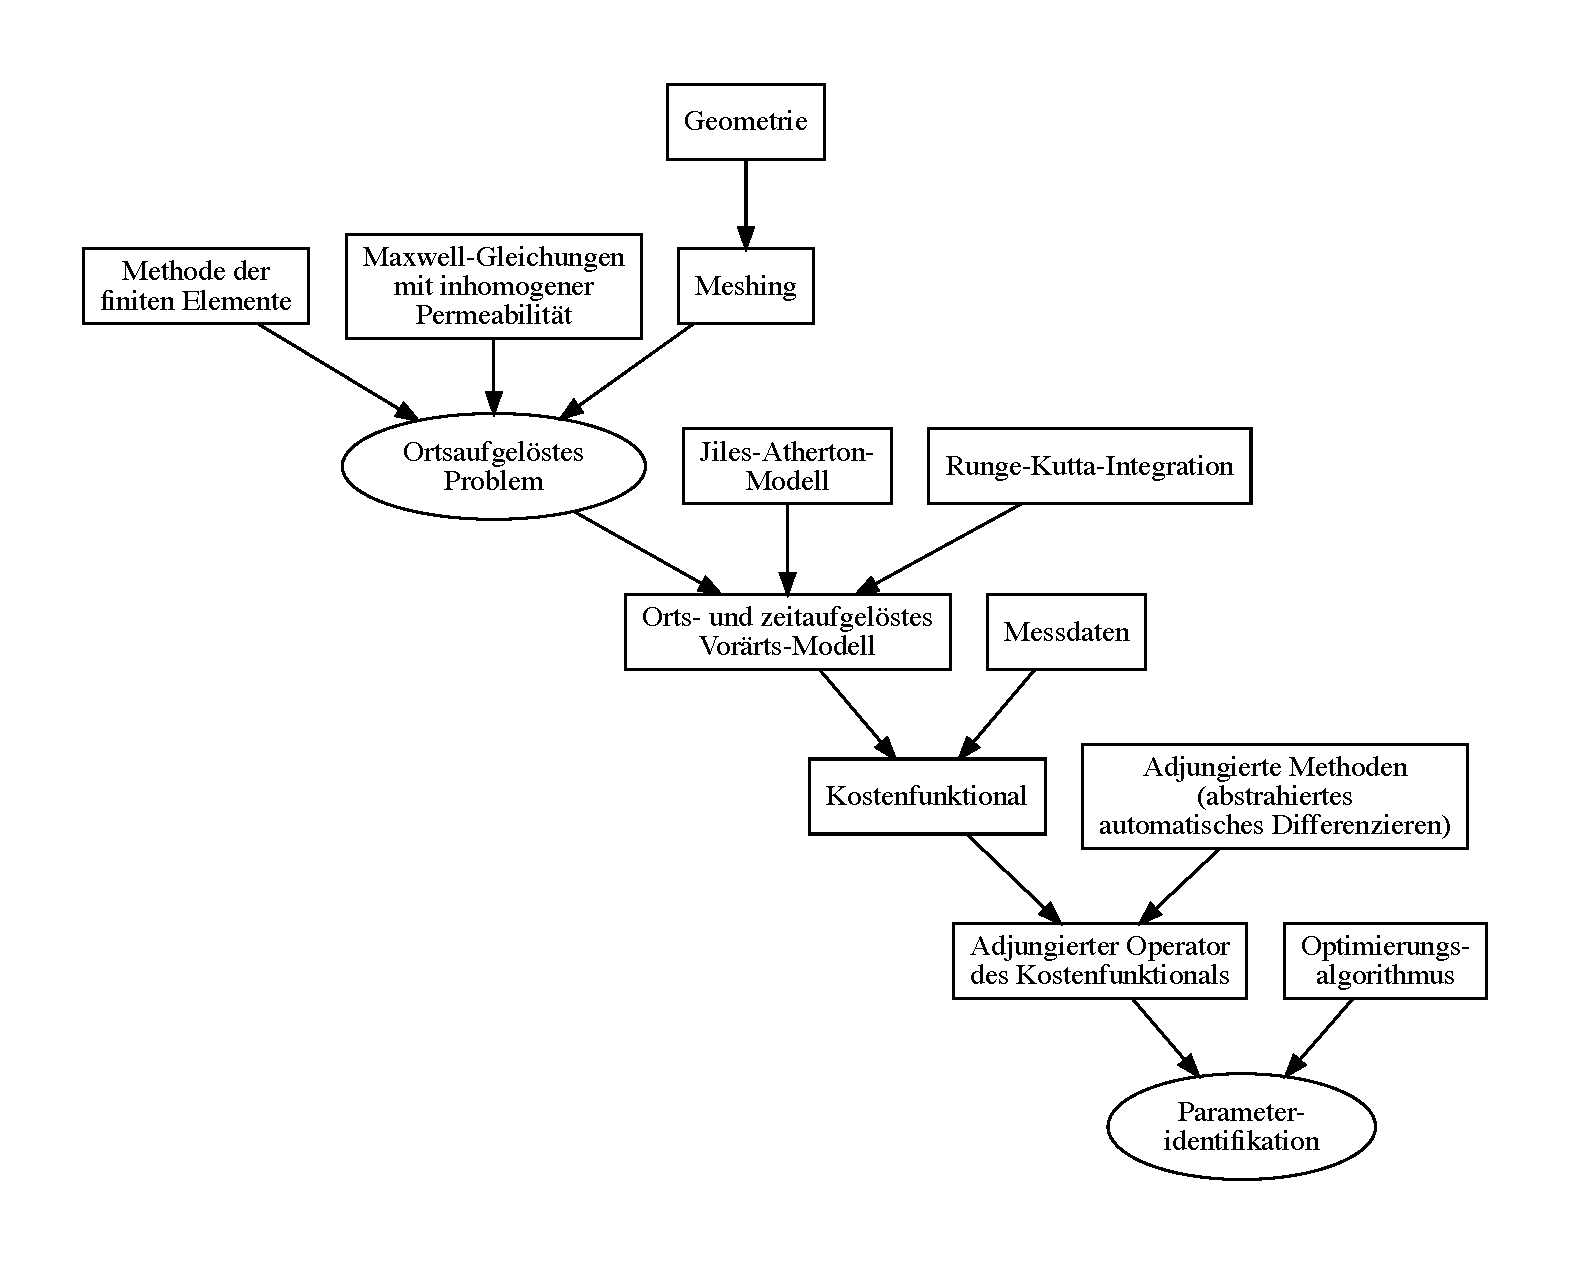
\includegraphics[width=\textwidth]{vorgehen_ort.pdf}

\end{figure}
\newpage
\printbibliography
\end{document}